\section{You graphical editor with Sirius}

%%%%
%%%%
\begin{frame}[allowframebreaks]{Create a first node}

	\smallblock{Create a first node}

	\begin{enumerate}
		\item on Default layer \ra new Diagram Element \ra new Node
		\item set id, domain class and semantic candidate expression of this node.
		\item Create a style for your node (eg. workspace image).
		\item Save and go to the opened diagram. All created streets are now visible.				
	\end{enumerate}	

	\framebreak

	\smallblock{Remark}
	If the Semantic Candidates Expression is not set, then all the streets in you project are selected. To fix that, set: {\bf feature:roads}. Now, only the roads of the current maps model are selected.

	\centering
	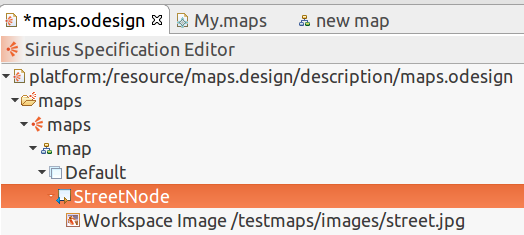
\includegraphics[scale=0.3]{figs/streetNode.png}

\end{frame}

%%%%
%%%%
\begin{frame}[allowframebreaks]{Create a conditional style node}

	Our goal here is to create a conditional style for Boulevard (horizontal or vertical Boulevard). For that we have two different images for Boulevard.

	\begin{enumerate}
		\item Create the Boulevard node
		\item Create a conditional style (set it to [ self.card = maps::cards::East or self.card = maps::cards::West  /])
		\item Create a style for this conditional style
		\item Create a second conditional style
	\end{enumerate}

	\centering
	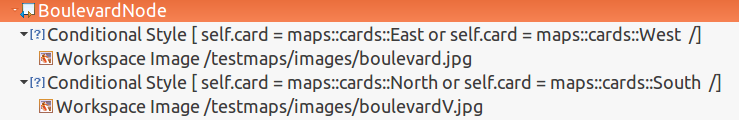
\includegraphics[scale=0.3]{figs/BoulevardNode.png}
	
\end{frame}

%%%%
%%%%
\begin{frame}[allowframebreaks]{Some other examples}

	\smallblock{Remark}
	
	You can find a completed example of a graphical editor created with Sirius (maps.odesign)


	\smallblock{More examples}
	
	In the completed example maps.odesign, you can find the following examples created:

	\begin{enumerate}
		\item Relation based Edge
		\item Palette creation of Node
		\item Palette creation of Relation based Edge
	\end{enumerate}

\end{frame}
